\chapter{条件语句和递归}

\section{ 模操作符}

\index{modulus operator 模操作符}
\index{operator!modulus 操作符!模}

模操作符用于两个整数,第一个操作数除以第二个操作数产生余数。在Python
中,模操作符是一个百分号(\verb"%")。语法的格式和其他的操作符相同。

\beforeverb
\begin{verbatim}
>>>quotient = 7 / 3
>>>print quotient
2
>>>remainder = 7 % 3
>>>print remainder
1
\end{verbatim}
\afterverb

7除以3等于2余1。\\

模操作符是非常有用的,比如,你可以查看一个数是否可以被另一个数整除---
如果{\tt x \% y}是0,{\tt x}就可以被{\tt y}整除。\\

\index{divisibility 整除}

你也可以用模运算来提取整数的最右边的数字。比如,{\tt x \% 10 }得到{\tt x}的最右面的一个数字\footnote{译注:个位数}(以十为底)。类似地,
{\tt x \% 100}得到最后的两位数字\footnote{十位和个位的数字}。

\section{布尔表达式}
\index{boolean expression 布尔表达式}
\index{expression!boolean}
\index{logical operator 逻辑运算符}
\index{operator!logical}

布尔表达式的结果要么是真(true),要么为假(false)。下面的例子是使用
{\tt ==}运算符,比较两个操作数,如果相等则结果为{\tt True},否则为{\tt False}:

\beforeverb
\begin{verbatim}
>>> 5 == 5
True
>>> 5 == 6
False
\end{verbatim}
\afterverb

{\tt True}和{\tt False}是两个特殊的值,属于{\tt bool}类型;他们不是
字符串:

\index{True special value True特殊值}
\index{False special value False特殊值}
\index{specail value!True}
\index{special value!False}
\index{bool type bool类型}
\index{type!bool}

\beforeverb
\begin{verbatim}
>>> type(True)
<type 'bool'>
>>> type(False)
<type 'bool'>
\end{verbatim}
\afterverb

{\tt ==}运算符是关系运算符中的一个,其他的还有:

\beforeverb
\begin{verbatim}
      x != y               # x is not equal to y
      x > y                # x is greater than y
      x < y                # x is less than y
      x >= y               # x is greater than or equal to y
      x <= y               # x is less than or equal to y
\end{verbatim}
\afterverb


尽管你可能很熟悉这些运算符,他们在Python中的表示方法和数学中的有很大
的不同。一个常见的错误是只使用一个{\tt =}号,而不是两个{\tt ==}号。
记住{\tt =}是赋值操作符,{\tt ==}是关系运算符。而且,Python中没有这样
的符号{\tt =<}或者{\tt =>}\footnote{在FP(functional programming中可能
会遇到这个符号}。

\index{relational operator 关系运算符}
\index{operator!relational}

\section{逻辑运算符}
\index{logical operator 逻辑运算符}
\index{operator!logical}

有三个逻辑运算符:{\tt and},{\tt or}和{\tt not}。这些操作符的意思和
在英语中的意思差不多。比如,{\tt x > 0 and x < 10}为真,仅当{\tt x}
大于0小于10\footnote{译注:在Python中,更pythonic的写法是 0 < x < 10
。  这样的符号对于c/c++背景的程序员来说,有点陌生,在c/c++等值的分别
是\&\&, || ,!}。

\index{and operator and运算符}
\index{or operator or运算符}
\index{not operator not运算符}
\index{operator!and}
\index{operator!or}
\index{operator!not}

如果{\tt n \% 2 == 0 or n \% 3 == 0}有一个条件语句为真,则表达式的值就为真,亦即n可以被2或3整除。\\

最后,{\tt not}运算符对一个布尔表达式取反,所以如果{\tt (
x > y)为假,则{\tt not (x > y)}为真,亦即,{\tt x}小于或等于{\tt y}。\\

严格来说,逻辑运算符的操作数只能是布尔表达式,但是Python
对此可没什么严格要求。任何不为0的整数也被解释成{\tt True}
\footnote{这个也可扩展到任何其他的类型,比如后面要涉及到的
list,tuple,dict,set还有str。}

\beforeverb
\begin{verbatim}
>>> 17 and True
True
\end{verbatim}
\afterverb

这个灵活性是很有用处的,但是可能会产生一些微妙的问题。我们
要尽可能的避免他们(除非知道自己在做什么)。

\section{条件执行}
\label{conditional execution}

\index{conditional statement 条件语句}
\index{statement!conditional}
\index{if statement if语句}
\index{statement!if}
\index{conditional execution 条件执行}

考虑到要写一些有用的程序,我们几乎总是需要检查条件,并改变相应的改变程序的行为。条件语句给了我们这个能力。最简单的要属{\tt if}语句了:



\beforeverb
\begin{verbatim}
if x > 0:
    print 'x is positive'
\end{verbatim}
\afterverb
{\tt if}语句后面的布尔表达式叫做条件。如果条件为真,则下面
缩进的语句就被执行。反之,则什么也不发生。\footnote{这是
针对本例而言,因为本例只有一条语句。在其他的情况下,可能
会有诸如{\tt else}之类的语句。}

\index{condition 条件}
\index{compound statment}
\index{statment!compound}

{\tt if}语句和函数定义有着相同的结构:
一个头,后面跟着一个缩进的语句块。这样的语句叫做复合语句。\\

虽然对复合语句里面可以含有的语句数量不限,但是必须至少有一
条\footnote{c/c++中没有这样的限制}。偶然地,可能在语句体里
暂时不需要语句(通常作为一个占位符)。在这种情况下,我们可以
使用{\tt pass}语句,它什么也不做。



\index{pass statement}
\index{statement!pass}

\beforeverb
\begin{verbatim}
if x < 0:
    pass          # need to handle negative values!
\end{verbatim}
\afterverb

\section{选择执行}
\label {alternative execution}

\index{alternative executive 选择执行}
\index{else keyword else关键字}
\index{keyword!else}

{\tt if}语句的第二种形式是选择执行,此时,有两种可能性,
条件决定了哪一个可能性被执行。语法是这样:

\beforeverb
\begin{verbatim}
if x%2 == 0:
    print 'x is even'
else:
    print 'x is odd'
\end{verbatim}
\afterverb

如果{\tt x}除以2的余数是0,我们可以判定{\tt x}是偶数,程序
就输出这个效果。如果条件为假,第二个语句就被执行。因为条件
必须为真或假,其中一个必定会被执行。选择项叫做分支,因为
它们是执行流的分支。

\index{branch 分支}


\section{链式条件}
\index{chained conditional 链式条件}
\index{conditional!chained}

有时,可能会有不止两种可能性,我们就需要更多的分支。一种方式是使用链式条件语句。

\beforeverb
\begin{verbatim}
if x < y:
    print 'x is less than y'
elif x > y:
    print 'x is greater than y'
else:
    print 'x and y are equal'
\end{verbatim}
\afterverb

{\tt elif}是"else if"的缩写形式。再次说明一下,只有一条
语句被执行。{\tt elif}语句的数目也是没有限制的。如果要写
{\tt else}语句,必须是在链式条件的最后,但是如果没有,也是
允许的。

\index{elif keyword elif关键字}
\index{keyword!elif}

\beforeverb
\begin{verbatim}
if choice == 'a':
    draw_a()
elif choice == 'b':
    draw_b()
elif choice == 'c':
    draw_c()
\end{verbatim}
\afterverb

每个条件按顺序被检查。如果第一个为假,下一个就被检查,如此
如此。如果有一个为真,相应的分支就被执行,链式语句也就终止
。尽管可能有多个条件为真,也只有第一个为真的分支被执行。\\


\section{嵌套的条件语句}
\index{nested conditional 嵌套的条件语句}
\index{conditional!nested}

一条条件语句也可以嵌套在另一个语句之中。我们写一个典型的例子:

\beforeverb
\begin{verbatim}
if x == y:
    print 'x and y are equal'
else:
    if x < y:
        print 'x is less than y'
    else:
        print 'x is greater than y'
\end{verbatim}
\afterverb
外层的条件包两个分支。第一个分支包含一个简单语句。第二个分支包含例外一个
{\tt if}语句,同时,这个{\tt if}语句也有两个分支。这两个简单的分之都是简
单语句,尽管他们本也可能是条件语句。\\

尽管缩进使得代码结构清晰,嵌套语句还是难以快速的理解。一般来说,尽可能的
避免使用嵌套条件语句。\\

逻辑运算符可以简化嵌套条件语句。比如,下面的代码可以只用一条条件语句:

\beforeverb
\begin{verbatim}
if 0 < x:
    if x < 10:
        print 'x is a positive single-digit number.'
\end{verbatim}
\afterverb

只有当我们“通过”了两个条件时,{\tt print}语句才会被执行,所以,我们可以用{\tt and}运算符达到同样的效果。

\beforeverb
\begin{verbatim}
if 0 < x and x < 10:
    print 'x is a positive single-digit number.'
\end{verbatim}
\afterverb
 


\section{递归}
\label{recusion}
\index{recursion 递归}


函数调用\footnote{译注:台湾的书籍一般翻译为呼叫,这个很形象}另外一个函数是合法的;函数调用他自身也是合法的。很难一眼看出这样做有什么好处\footnote{译者注:我猜,这种情况就像是自己把自己提起来一样~~},但实践证明,
这是程序能做的最具有魔力的事情之一。比如,看下面的函数:

\beforeverb
\begin{verbatim}
def countdown(n):
    if n <= 0:
        print 'Blastoff!'
    else:
        print n
        countdown(n-1)
\end{verbatim}
\afterverb

如果{\tt n}是非正数,程序输出,“Blastoff!“,否则,输出{\tt n},然后调用
{\tt countdown}函数---也就是它自己---同时把{\tt n-1}当作参数传递给它。

如果我们调用这个函数,究竟发生了什么?

\beforeverb
\begin{verbatim}
>>> countdown(3)
\end{verbatim}
\afterverb
%
{\tt countdown}从{\tt n=3}开始执行,{\tt n}此时大于0,于是输出3,接着
调用自身。。。。。。

\begin{quote}
{\tt countdown}从{\tt n=2}开始执行,{\tt n}此时大于0,于是输出2,接着调用自身。。。。。。

\begin{quote}
{\tt countdown}从{\tt n=1}开始执行,{\tt n}此时大于0,于是输出1,接着调用自身。。。。。。

\begin{quote}
{\tt countdown}从{\tt n=0}开始执行,{\tt n}此时不大于0,输出“Blastoff!"
然后返回。
\end{quote}

接受{\tt n=1}的{\tt countdown}返回。
\end{quote}

接受{\tt n=2}的{\tt countdown}返回。
\end{quote}

%接受{\tt n=3}的{\tt countdown}返回。
%\end{quote}

{\tt countdown}接受{\tt n=3}的函数返回。

然后,我们就会到\verb"__main__"里了。整个输出如下:

\beforeverb
\begin{verbatim}
3
2
1
Blastoff!
\end{verbatim}
\afterverb

 调用自身的函数称作递归函数;调用的过程叫做递归。

 \index{recursion 递归}
 \index{function!recursive}

另外一个例子,我们写一个打印一个字符串{\tt n}次的函数。

\beforeverb
\begin{verbatim}
def print_n(s, n):
    if n <= 0:
        return
    print s
    print_n(s, n-1)
\end{verbatim}
\afterverb

如果{\tt n <= 0},{\tt return}语句退出函数。执行流立刻返回到调用者,
剩余的部分就不再被执行了。

\index{return statement return语句}
\index{statement!return}

函数的剩余部分和{\tt countdown}还书相似:如果{\tt n}大于0,输出{\tt s},然后调用自身显示{\tt s} $n-1$次。所以,输出的行数是{\tt 1 + (n-1)},
也就是{\tt n}次。\\

这样简单的例子,其实可以很容易用一个{\tt for}循环来实现。但我们以后将会看
到很难写成{\tt for}循环形式,但是很容易用递归实现的例子,我们现在就
开始认识递归是有好处的。

{\section{递归函数的堆栈图}
\index{stack diagram 堆栈图}
\index{function frame 函数图}
\index{frame 图}
 
在\ref{堆栈图}部分,我们使用堆栈图代表程序在函数调用过程中的状态。
同样的方法也可以帮助我们理解递归函数。\\

每次函数调用的时候,Python创建一个新的函数框图,里面包含了函数的局部
变量和参数。对于递归函数来说,可能会有不止一个框图同时出现在堆栈图里
。\\

下图显示了{\tt n = 3}时{\tt countdown}函数的堆栈图。

\beforefig
\centerline{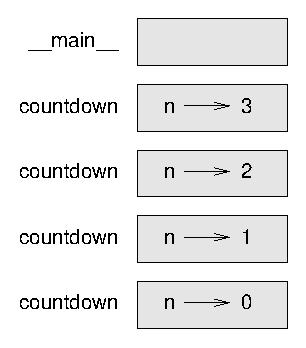
\includegraphics{figs/stack2.eps}}
\afterfig

像通常的一样,栈顶是\verb"__main__"的卡框图。由于我们没有在\verb"__main__"里创建任何的变量或传递任何的参数给它,所以它是空的。

\index{base case 终止条件}
\index{recursion!base case}

四个{\tt countdown}框图拥有不同的{\tt n}值。栈底,{\tt n = 0},叫做
终止条件(base case)。不执行任何的递归调用,所以就没有更多的框图了。

\begin{quote}
画\verb"print_n"的堆栈图,其中,\verb"s = 'Hello'" {\tt n = 2}。
\end{quote}

\begin{quote}
编写\verb"do_n"函数,接受一个函数对象,和一个数字,{\tt n}作为参数,调用传递过来的函数{\tt n}次。
\end{quote}

\section{无穷递归}
\index{infinite recursion 无穷递归}
\index{recursion!infinite}
\index{runtime error 运行时错误}
\index{error!runtime}
\index{traceback 跟踪}

如果递归函数没有终止条件,就会无止境的递归\footnote{译者:直到消耗完资源,或者操作系统终止它}。当达到最大递归深度时,Python就会报告错误
信息。

\index{exception!RuntimeError}
\index{RuntimeError}

\beforeverb
\begin{verbatim}
  File "<stdin>", line 2, in recurse
  File "<stdin>", line 2, in recurse
  File "<stdin>", line 2, in recurse
                  .   
                  .
                  .
  File "<stdin>", line 2, in recurse
RuntimeError: Maximum recursion depth exceeded
\end{verbatim}
\afterverb

这个追踪比我们上一章看到的要大很多。当错误产生时,在栈中有1000张{\tt recurse}框图!

\section{键盘输如}
\index{keyboard input 键盘输入}

迄今为止,我们编写的程序对用户来说有点“不礼貌”---不接受来自用户的输入。每次只是做同样的事。\\

Python提供了一个内置的函数\verb"raw_input"获取用户的输入\footnote{在
Python3.0中,这个函数叫做{\tt input}。  译注:在Python3.x中都是如此}
当\verb"raw_input"函数被调用时,程序停下来等待用户输入些东西。当用户敲击{\sf Return}或者{\sf Enter},程序恢复运行,\verb"raw_input"把用户输入的东西作为字符串返回。

\index{Python 3.0}
\index{raw\_input function raw\_input函数}
\index{function!raw\_input}


\beforeverb
\begin{verbatim}
>>> input = raw_input()
What are you waiting for?
>>> print input
What are you waiting for?
\end{verbatim}
\afterverb

 在用户输入之前,最好能够输出一个提示,告诉用户输入什么。\verb"raw_input"可以接受一个提示作为参数。

\index{prompt 提示}

\beforeverb
\begin{verbatim}
>>> name = raw_input('What...is your name?\n')
What...is your name?
Arthur, King of the Britons!
>>> print name
Arthur, King of the Britons!
\end{verbatim}
\afterverb

提示后面的\verb"n"代表一个换行,这是一个特殊字符,产生一个断行。
这也是为什么用户的输入出现在提示下面的原因。

\index{newline 换行}

如果希望用户输入一个整数,可以尝试把返回值转换为{\tt int}。

\beforeverb
\begin{verbatim}
>>> prompt = 'What...is the airspeed velocity of an unladen swallow?\n'
>>> speed = raw_input(prompt)
What...is the airspeed velocity of an unladen swallow?
17
>>> int(speed)
17
\end{verbatim}
\afterverb

但是,如果用户输入的不是数字组成的字符串,就会得到一个错误:

\beforeverb
\begin{verbatim}
>>> speed = raw_input(prompt)
What...is the airspeed velocity of an unladen swallow?
What do you mean, an African or a European swallow?
>>> int(speed)
ValueError: invalid literal for int()
\end{verbatim}
\afterverb

我们以后将会看到如何处理这样的错误。

\index{ValueError }
\index{exception!ValueError}


\section{Debugging 调试}
\label{whitespace}
\index{debugging 调试}
\index{traceback 跟踪}

当错误发生,Python 输出的跟踪信息,包含大量的信息,但是也很容易让人
“眼花缭乱”,特别是栈中有很多框图的时候。最有用的部分通常是:

\begin{itemize}

\item 什么类型的错误

\item 在什么地方发生的

\end{itemize}

 通常,语法错误很容易发现,但是也有些微妙的东西\footnote{原文是:but 
there are a few gotchas}。“空格”错误可能很微妙,因为空格和制表是不可见的,而且我们习惯上忽略它们\footnote{特别是在不同的机器上,或者不同
的工具上大开源码的时候}。

\index{whitespace 空格}

 
\beforeverb
\begin{verbatim}
>>> x = 5
>>>  y = 6
  File "<stdin>", line 1
    y = 6
    ^
SyntaxError: invalid syntax
\end{verbatim}
\afterverb

这个例子中,问题发生在第二行有了一个空格缩进。但是错误指向了{\tt y},
这个是一个误导。一般,错误信息提示问题发生的地方,当时实际的错误可能
在提示的前面一点,有时在前一行。

\index{error!runtime}
\index{runtime error 运行时错误}

对于运行时错误,也是如此。假设,你想用分贝计算信噪比。公式是$SNR_{db} = 10 \log_{10} (P_{signal} / P_{noise})$。你可能写出如下的Python代码:

\beforeverb
\begin{verbatim}
import math
signal_power = 9
noise_power = 10
ratio = signal_power / noise_power
decibels = 10 * math.log10(ratio)
print decibels
\end{verbatim}
\afterverb
但是,当你运行时,你会得到一个错误信息\footnote{在Python3.0中,不会
得到错误信息;除法运算符执行浮点除,尽管操作数是整数,这个和实际
很贴近}。

\index{exception!OverflowError}
\index{OverflowError}

\beforeverb
\begin{verbatim}
Traceback (most recent call last):
  File "snr.py", line 5, in ?
    decibels = 10 * math.log10(ratio)
OverflowError: math range error
\end{verbatim}
\afterverb

错误信息提示错误发生在第五行,但是那行根本没有错误。为了发掘出真正的错误,打印{\tt ratio}的值可能会有帮助,结果显示是0。问题出现在第四行,因为两个整数的除法实施的是地板除(floor division)\footnote{译注:
Python核心编程的中译本中,把它翻译成地板除}。解决方案是用浮点数来表示
信号功率和噪声功率。

\index{floor division 地板除}
\index{division!floor}

总的来书,错误信息告诉我们出现问题的地方,但通常不是问题发生的根本所在。

\section{术语表}

\begin{description}

\item [modulus operator 模运算符:] 一个操作符,记法为百分号({\tt \%})。作用在两个整数之间,产生余数。
\index{modulus operator 模运算符}
\index{operator!modulus}

\item [boolean expression 布尔表达式:]值要么为{\tt True}要么为{\tt False}的表达式。
\index{boolean expression 布尔表达式}
\index{expression!boolean}

\item [relational operator 关系运算符:] 比较操作数的的运算符:
{\tt ==},{\\t !=},{\tt >},{\tt <},{\tt >=}和{\tt <=}。

\item [logical operator 逻辑运算符:]连接布尔表达式的运算符:
{\tt and},{\tt or}和{\tt not}。

\item [conditional statement 条件语句:]依靠一些条件控制执行流的语句。
\index{conditional statement 条件语句}
\index{statement!conditional}

\item [condition 条件:] 条件语句中的布尔表达式,决定分支的执行。
\index{condition 条件}

\item [compound statement 复合语句:]包含头和体的语句。头一(:)结尾,体依据头,缩进。
\index{compound statement}

\item [body 体:] 符合语句中的一系列语句。
\index{body}

\item [branch 分支:]条件语句中的可选择执行的语句(序列)。
\index{branch}

\item [chained conditional 链式条件语句:] 拥有一系列的选择分之的条件语句。
\index{chained conditional 链式条件语句}
\index{conditional!chained}

\item [nested conditional 嵌套条件语句:]出现在条件语句中分分支中的条件语句。
\index{nested conditional 嵌套条件语句}
\index{conditional!nested}

\item[recursion 递归:]调用函数自身的过程。
\index{recursion 递归}

\item[base case 终止条件:] 递归函数里的一个条件分支,终止递归调用。
\index{base case}

\item[infinite recursion 无穷递归:]没有终止条件的递归,最终无穷递归产生一个运行时错误。
\index{infinite recursion 无穷递归}

\end{description}

\section{练习}

\begin{ex}
\index{Fermat's Last Theorem费马最后定理}


费马最后定理这么表述:不存在这样的整数$a$,$b$和$c$使得对于$n$大于2,\[ a^n + b^n = c^n \]。
\begin{enumerate}

\item 编写\verb"check_fermat"函数,接受4个参数---{\tt a},{\tt b},{\tt c}和{\tt n}---验证费马定理是否正确。如果$n$大于2,\[a^n + b^n = c^n \]是成立的,程序输出,``Holy smokes, Fermat was wrong!'',否则,输出,``No, that doesn't work.''

\item 编写一个函数提示用户输入 {\tt a}, {\tt b}, {\tt c} and {\tt n}的值,把他们转换成整数,使用\verb"check_fermat"验证是否违背费马定理。

\end{enumerate}
\end{ex}


\begin{ex}
\index{triangle 三角形}

给你三根木棒,你也许能,也许不能组成一个三角形。比如,其中一根木棒12英尺长,其他的两根是1英尺长,很明显,不能使短木棒在长木棒的中间相遇。
对于三个任意长度,可以用一个简单的测试在检测是否能够构成一个三角形。

\begin{quotation}
“如果三个长度的任意一个大于其他两个之和,就不能构成一个三角形。否则,就可以\footnote{如果两个长度之和等于第三个,他们形成退化的三角形。}“
\end{quotation}


\begin{enumerate}

\item 编写\verb"is_triangle"函数,接受3个整数作为参数, 依据能不能构成三角形,输出要么是“Yes“,要么是“or“。

\item 编写一个函数提示用户输入木棒的长度,转换成整数,然后调用\verb"is_triangle"检测是否可以构成一个三角形。

\end{enumerate}

\end{ex}

接下来的练习使用\ref{turtlechap}章节的TurtleWorld。

\index{TurtleWorld}
\begin{ex}

阅读下面的函数,看看它的功能是什么。然后运行它(查看\ref{turtlechap}章节的例子)。

\beforeverb
\begin{verbatim}
def draw(t, length, n):
    if n == 0:
        return
    angle = 50
    fd(t, length*n)
    lt(t, angle)
    draw(t, length, n-1)
    rt(t, 2*angle)
    draw(t, length, n-1)
    lt(t, angle)
    bk(t, length*n)
\end{verbatim}
\afterverb

\end{ex}

\begin{ex}
\index{koch curve 柯霍曲线}

柯霍曲线是一个分形体,看起来像这样:

\beforefig
\centerline{
\includegraphics[height=1in]{figs/koch.eps}}
\afterfig

画长度为$x$的柯霍曲线,你所需要做得就是
\begin{enumerate}

\item 画一个长度为$x/3$的柯霍曲线

\item 左转60度。

\item 画一个长度为$x/3$的柯霍曲线

\item 右转120度

\item 画一个长度为$x/3$的柯霍曲线

\item 左转60度。

\item 画一个长度为$x/3$的柯霍曲线

\end{enumerate}

唯一的例外是如果$x$小于3,此时,就直接画一个长度为$x$的直线。

\begin{enumerate}

\item 编写{\tt koch}函数,接受一个turtle和长度作为参数,使用turtle画
一个给定长度的柯霍曲线。

\item 编写{\tt snowflake}函数,画3个柯霍曲线,形成雪花的轮廓。

可以查看我的答案\url{thinkpython.com/code/koch.py}。

\item 柯霍曲线可以用多种方式一般化。查看\url{wikipedia.org/wiki/Koch_snowflake}例子,并实现自己喜欢的雪花。

\end{enumerate}
\end{ex}




